In this example of acrobatic sports biomechanics, the goal was to maximize the twist rotation ($\phi$) of a 8-DoF model in a backward somersault.
The model was composed of a 6-DoF root segment and two 1-DoF torque actuated shoulder joints.
Two different numerical description of the root segment rotations were used (Euler angles and quaternions).
The objective function was as follows:

\begin{eqnarray}\label{eq:ocp_Trampo}
\mathcal{J} = \omega_1 \underbrace{\int_0^T \dot{\phi}~dt}_{\mathtt{MIN\_TWIST}}  +~\omega_2 \underbrace{\int_0^T \sum_{i=1}^{2}~\tau_{i}^2~dt}_{\mathtt{MIN\_ TORQUE}},
\end{eqnarray}
with $\omega_1 = -1$ (resulting in the maximization of the first term) and $\omega_2 = 1\times 10^{-6}$, T the duration of the movement and $\tau_{i}$ the torque control input of the $i^{th}$ arm DoF.
The first term of the objective function (Eq.~\ref{eq:ocp_Trampo}) corresponds to maximizing the twist velocity and the second term serves as control regularization.


The movement lasted for approximately 1 second and was discretized with 80 shooting nodes.
The solutions for both models were \comment{similar}{ce n'est pas vraiment le cas, commenter} (Fig.~\ref{fig:snapshots_quaternion_base_twisting_somersault}) highlighting the equivalence of the two rotation representations.
Euler angles have the advantage to be easily interpretable, but they suffer from the loss of a DoF at the Gimbal lock (leading to numerical instabilities).
The use of a quaternion-based representation is tackles this numerical stability issue when a joint is free to rotate on a three-dimensional range of motion.
Quaternion's integration must be handled with care~\cite{bailly2020optimal}, which was taken care of in \textit{bioptim}.


\begin{figure*}[t!]
\centering
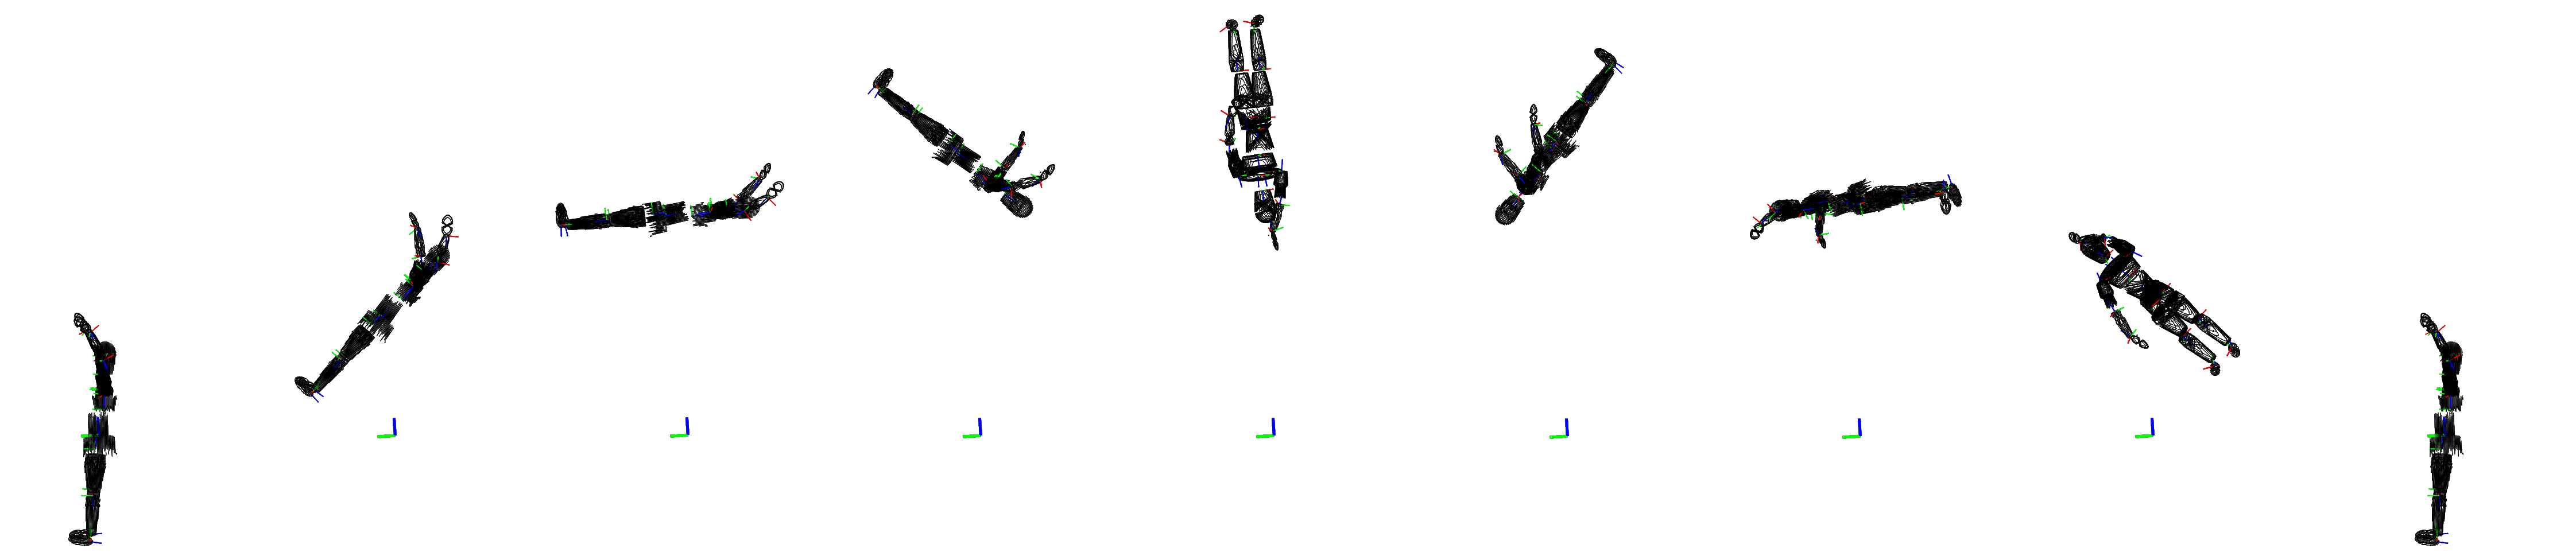
\includegraphics[width=\textwidth]{figures/Euler_Bioptim_MaxVrille_dos.png}\\
\vspace*{0.5em}
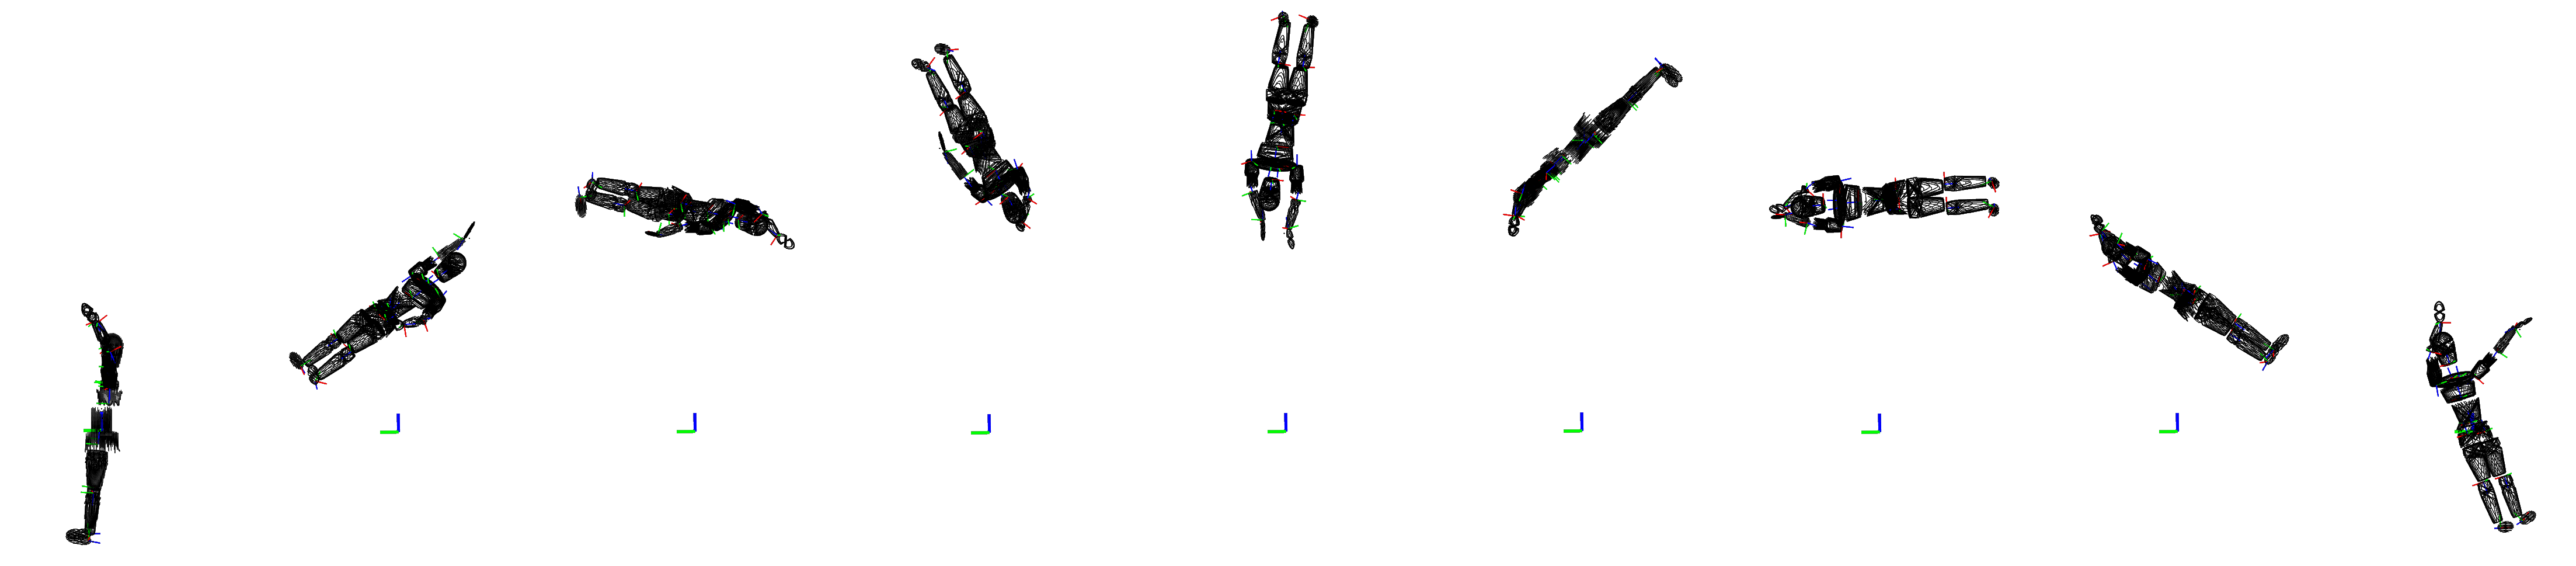
\includegraphics[width=\textwidth]{figures/Quat_Bioptim_MaxVrille_dos.png}
\caption{Snapshots of a maximally twisting somersault driven by shoulder torque actuators and a free base expressed by Euler angles (top) or quaternions (bottom).}
\label{fig:snapshots_quaternion_base_twisting_somersault}
\end{figure*}


% \begin{table}[h!]
% \caption{\small Objective terms of quaternion base maximally twisting somersault}
% \label{tab:Quaternion_base_twisting_somersault}
% \centering
% \begin{tabular}{c c c c}
% \toprule 
% & Type & Function & Weight \\ 
% \midrule
% $\#1$ & Lagrange & MINIMIZE\_TWIST & $-1e1$ \\ 
% \midrule
% $\#2$ & Lagrange & MINIMIZE\_ TORQUE & $1e-6$ \\ 
% \bottomrule
% \end{tabular}
% \end{table}













